\section{\SecAdvanceNesting} \label{sec:nest_exp}
%====================================================================================

ネスティングとは、領域が重複するように複数の計算領域を入れ子(ネスト)構造に設定する方法である。
図\ref{fig_nestsample}は、3つの領域を用いたネスティングの例を示している。
外側の領域は、大きな空間スケールの現象を表現するため、低い水平解像度で広い領域を設定する。
一方、内側の領域は、小さな空間スケールの現象を解像するために、狭い範囲であるが高い水平解像度に設定する。
外側の領域の計算結果は、内側の領域に対する境界値データとして用いられる。
ここでは、
データを渡す外側の領域を「親領域」、データを受ける内側の領域を「子領域」と呼ぶことにする。

ネスティングの方法は下記のように分類される。
\begin{itemize}
\item 実行方法
\begin{description}
 \item[オンライン・ネスティング]\mbox{}\\
計算途中で親領域と子領域の情報を交換しながら、親領域と子領域の計算を同時に実行する方法。
 \item[オフライン・ネスティング]\mbox{}\\
最初に親領域の計算を行って子領域用の初期値・境界値を作成し、
その後に子領域の計算を行う方法。
\end{description}
\item データの受け渡し方法
\begin{description}
 \item[一方向ネスティング]\mbox{}\\
親領域は子領域にデータを送るが、子領域は親領域にデータを送らない。
%つまり、データの流れは親領域から子領域に向かう一方通行。
親領域の結果は、子領域の結果の影響を受けない。
 \item[双方向ネスティング]\mbox{}\\
親領域は子領域にデータを送り、子領域からのデータも受け取る。
したがて、二つの領域の計算は互いに影響し合う。
この方法はオンランイン・ネスティング時に適用できるが、
{\scalerm} v{\version} ではまだ実装されていない。
\end{description}
\end{itemize}

オンラインとオフラインの違いは、親領域から子領域にデータを与える更新頻度にある。
オンライン・ネスティング実験では、子領域の境界条件は親領域の時間刻み幅($\Delta t$)毎に更新される。
オフライン・ネスティング実験では、更新頻度は親領域の計算におけるヒストリファイルの出力間隔に依存する。

ネスティングがオフラインかオンラインかに関わらず、親領域と子領域の格子間隔比($\mathrm{DX}_{\mathrm{d01}}/\mathrm{DX}_{\mathrm{d02}}$)に関してコードの実装上の制限はない。
ただし、この比率が大きすぎると計算結果の物理性能が下がる可能性がある。
\scalerm では、5倍以下で使用することを推奨する。

本節では、親領域の設定ファイルを\verb|***.d01.conf| 、子領域の設定ファイルを\verb|***.d02.conf| と表記する。

\begin{figure}[t]
\begin{center}
  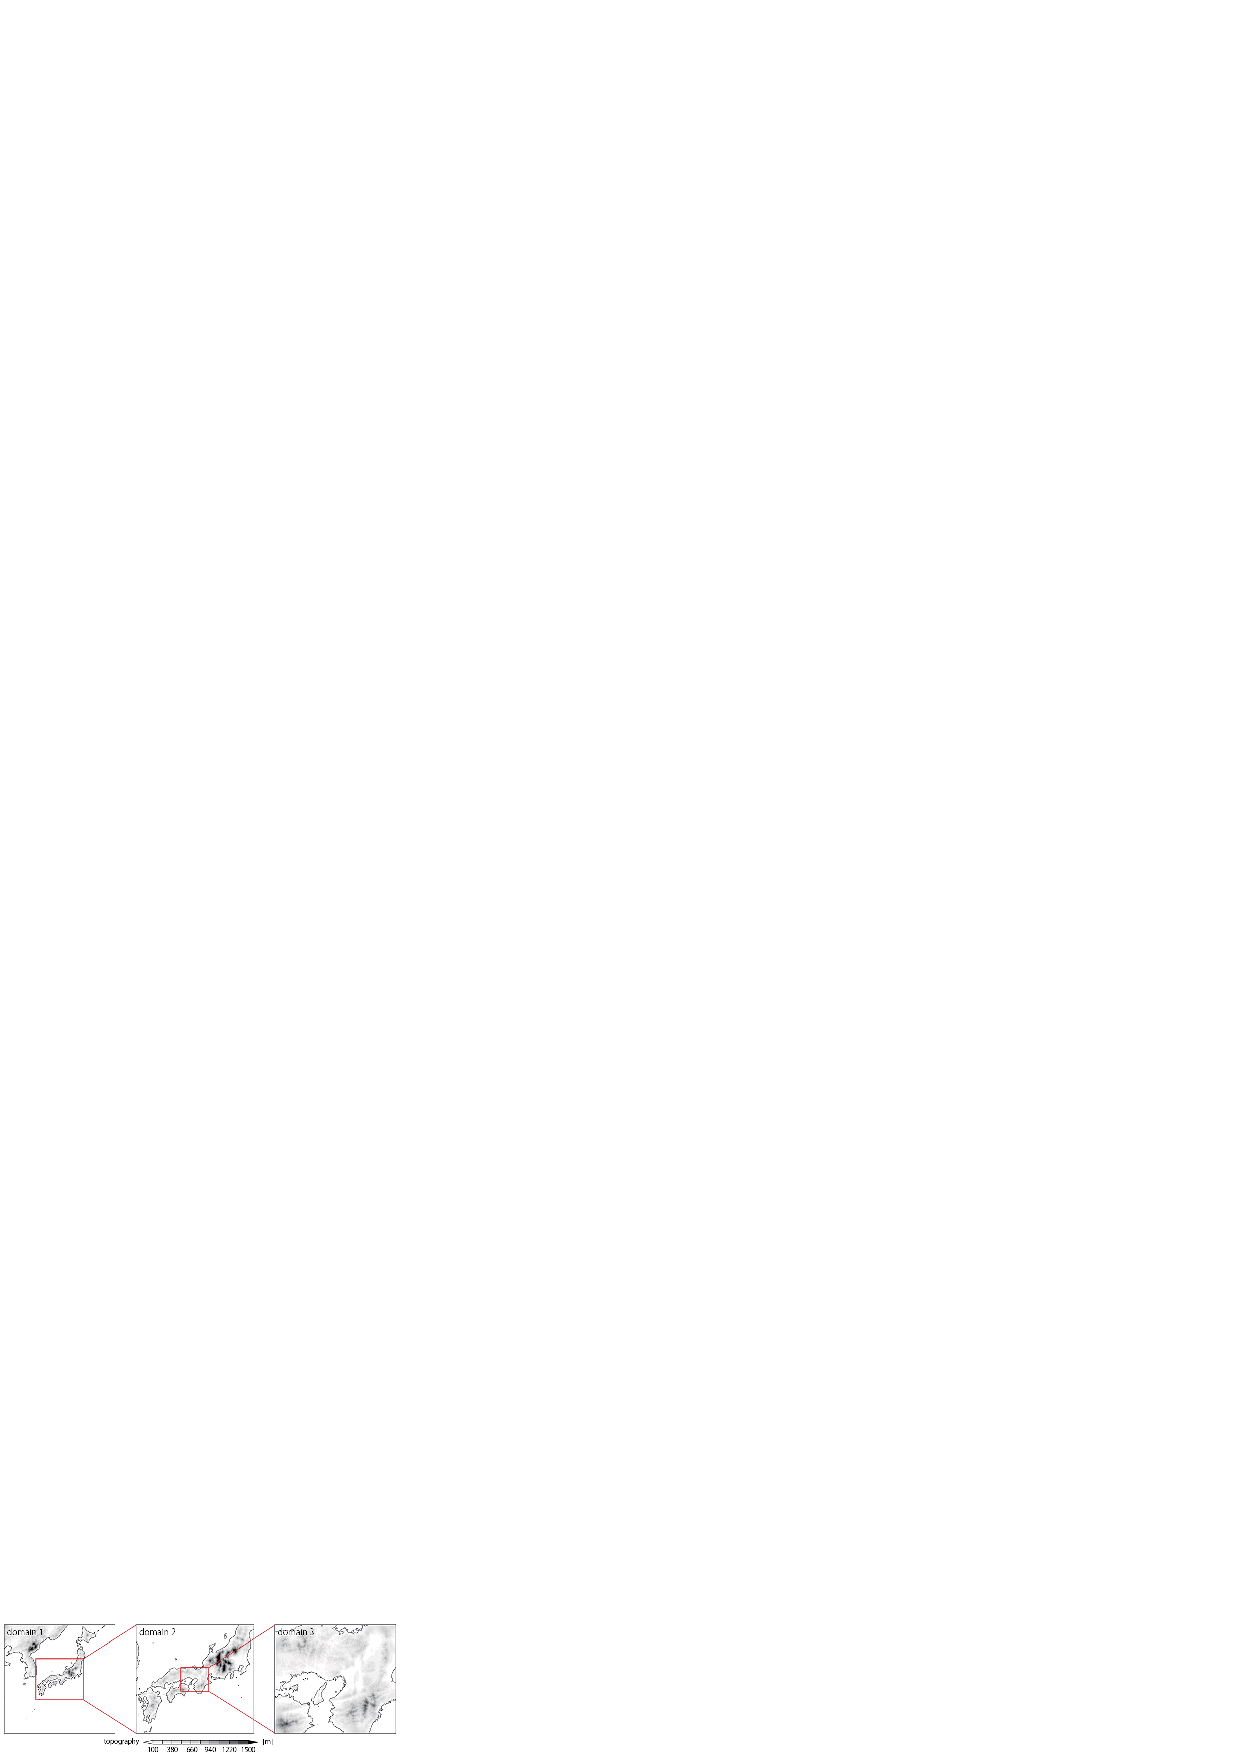
\includegraphics[width=1.0\hsize]{./../../figure/nesting_sample.pdf}\\
  \caption{西日本を対象とした領域ネスティングの例。
    domain 1が最外領域でdomain 3が最内領域である。
    赤い矩形と線は、領域の位置や他の領域との関係を示している。
    水平格子間隔は domain 1 では 7.5 km、domain 2 では 2.5 km、
    domain 3 では 0.5 kmである。}
  \label{fig_nestsample}
\end{center}
\end{figure}
